\section{Model architecture}
\label{sec:model_architecture}

In the process of this thesis, two versions of the FESD model were implemented. The first approach can be seen in Figure \ref{fig:model_architecture_v1}. In the first approach, the RGB, Depth, and Joint data are passed into three different convolutional neural networks with intermittent max-pooling. The output of the three networks is then concatenated and passed into three fully connected layers. The output of the fully connected layers is a 1D 2, 4, 20, and 80 tensors of multi-object multi-class values depending on the problem set. The different problem sets are discussed in section \ref{sec:problem_set}. However, for this approach, the amount of data that was captured was not sufficient so no satisfying results could be achieved. Therefore, a second approach was implemented.

The second approach is relying on transfer learning, in which a pretrained model is use

\begin{figure}[h]
  \centering
  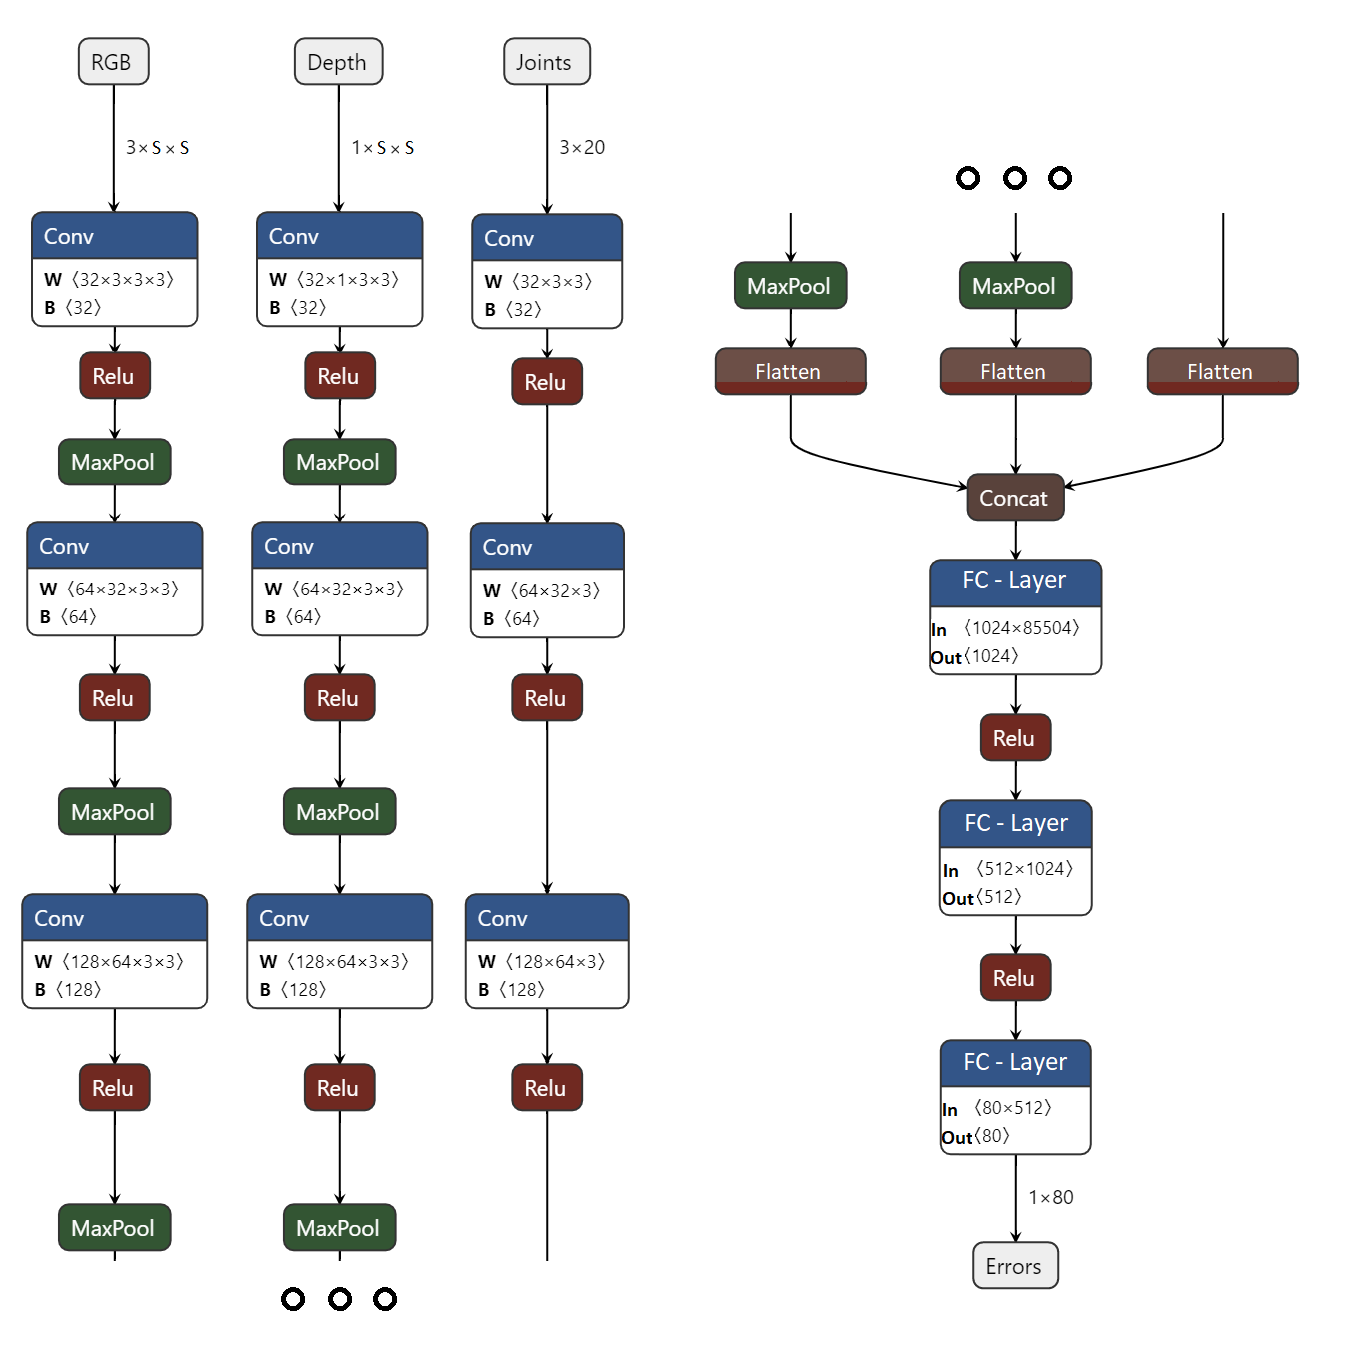
\includegraphics[width=\linewidth]{figures/Model/FESD.png}
  \caption[FESDModel architecture version 1]{Original FESDModel architecture with three different inputs; RGB, Depth and Joint data. After three convolutions the three streams are concatenated to be passed into three fully connected layers. The output is a 1D 80 tensor of multi-object multi-class values.}
  \label{fig:model_architecture_v1}
\end{figure}

% With the data prepared and the data layout known, we can start to build a model to predict the errors in the data. As is common practice in computer vision tasks, we use a convolutional neural network to predict the error type of the individual joints. The input of the network are the individual datastreams, i.e. a stream of RGB data, a stream of depth data, and a stream of joint data. The output of the network is a list of error labels for each joint. The network is trained to predict the error labels for each joint. The error labels are the same as the error labels used in the data labeling. The error labels are explained in section \ref{sec:data_labeling}. 

% The different modalities are combined in the final three fully connected layers. The model architecture is shown in figure \ref{fig:model_architecture}.


% We pass the three different modalities as multi dimensional tensors into the network. Prior to this we applied all augmentations and resize the images to fit the tensor size as seen in Figure \ref{fig:model_architecture}. We discuss the augmentations that we apply in Section \ref{sec:data_augmentation}.

% Then a 3x3 convolution is applied on the data to extract low level features. After the features are extracted a Relu, or rectified linear unit is applied to combat the vanishing gradient problem. For the visual channels of the data, i.e. the RGB data and the depth data MaxPooling is applied to down sample the data. It is not applied to the joint data since the data available per input is already limited.

% This Convolution, Relu and Max Pooling is repeated three times to extract ever higher level features. We found that three layers were the best choice.

% After the convolution layers we flatten the output of each of the RGB, Dept and Joint CNN into a single feature vector. This feature vector is passed into the fully connected network. We use three layers to gradually reduce the neuron size to our desired output size of $20\cdot4$ classes.

% Inherently this is the network, however, to use the data a softmax is applied to each object to extract the most likely joint error. The $20\cdot4$ classes can then be reduced to $20$ errors and a confidence rating.